\documentclass[letterpaper,11pt]{article}
\usepackage[spanish]{babel}
\usepackage[utf8]{inputenc}
\usepackage{graphicx}
\usepackage{amsfonts,amsmath,amssymb,float, amsthm,mathrsfs}  
\usepackage[right=4.5cm,left=2cm,top=3cm,bottom=3cm,headsep= 0.7cm,footskip=0.5cm]{geometry}
\usepackage{enumerate}
\usepackage{wrapfig} 
\usepackage[rflt]{floatflt} 
\usepackage{framed}
%\usepackage[most]{tcolorbox}
\usepackage[dvipsnames]{xcolor}
\colorlet{shadecolor}{green!20}
\setlength\FrameSep{0.5ex}
\usepackage{thmtools}
\usepackage{esint}
\usepackage{cancel}
\usepackage{listings} 
\usepackage{pstricks, caption}
\usepackage[colorlinks]{hyperref}
\usepackage{csquotes}
\usepackage{fullpage}
\usepackage{enumitem}
\usepackage{etoolbox}
\usepackage{tikz}
\usepackage{tikz-3dplot}
\tdplotsetmaincoords{80}{70}
\usetikzlibrary{decorations.markings}
\usetikzlibrary{arrows,babel}
\usepackage[font=small]{caption}
\usepackage{scalerel} %\scaleto{text}{size}
\usepackage{subfigure}
\usepackage{fancyhdr}
\usepackage{comment}
\usepackage{marginnote}
\usepackage{tensor}
\usepackage{cleveref}
\newcommand{\dbar}{\mathchar'26\mkern-12mu d}
\renewcommand*{\marginnotevadjust}{-0.1cm}
\renewcommand*{\marginfont}{\footnotesize}
\setlength{\headheight}{15pt}
\addtolength{\topmargin}{-14.49998pt}
\setlength{\headsep}{15pt}
\setlength{\footskip}{14.49998pt}
\decimalpoint
\newcommand{\grad}{^\circ}
\newlength{\drop}
\DeclareMathOperator{\sign}{sgn}
\DeclareMathOperator{\Log}{Log}
\providecommand{\norm}[1]{\lVert#1\rVert}

\let\cancelorigcolor\CancelColor% Just for conveniency...

\newcommand{\CancelTo}[3][]{%
  \ifblank{#1}{}{%
    \renewcommand{\CancelColor}{#1}%
  }
  \cancelto{#2}{#3}% 
}


\begin{document}

\pagestyle{plain}

\begin{flushleft}\vspace{-2cm}
Departamento de Física \\
Facultad de Cs. Físicas y Matemáticas\\
Universidad de Concepción
\end{flushleft}

\begin{flushright}\vspace{-1.5cm}
\textbf{Tópicos en Relatividad General} 
\end{flushright}



\rule{\linewidth}{0.1mm}

\begin{center}
\textbf{\LARGE Semana 3}
\end{center}

\begin{flushleft}
\textbf{Nombre:} Alejandro Saavedra San Martín. \\
\textbf{Profesor:} Guillermo Rubilar Alegría.
\end{flushleft}

Concluímos que las geodésicas tipo tiempo en la geometría de Schwarzschild quedan completamente determinados resolviendo la siguiente ecuación para $r = r(\tau)$.
\begin{equation} \label{eq:geodesic-time-1}
\dot{r}^2 = k^2 c^2 - c^2 \left(1 - \frac{2m}{r}\right) \left( 1 + \frac{h^2m^2}{r^2} \right).
\end{equation}

Si definimos el \textbf{potencial efectivo}
\colorlet{shadecolor}{green!20}
\begin{shaded}
\begin{equation}
\tilde{V}(r) := \left( 1 - \frac{2m}{r}\right) \left(1 + \frac{h^2m^2}{r^2} \right),
\end{equation}
\end{shaded}

de modo que \eqref{eq:geodesic-time-1}
 puede reescribirse como
 \begin{equation} \label{eq:geodesic-time-2}
 	\frac{\dot{r}^2}{c^2} = k^2 - \tilde{V}(r).
 \end{equation}
 
 Esta elección del potencial es motivada por la condición de conservación de la energía mecánica de un cuerpo no-relativista:
\begin{equation}
 v^2 = \frac{2}{m}(E-V). 
\end{equation}
 
 Al igual que en el problema de Keplerm, la relación \eqref{eq:geodesic-time-2} restringe los valores para la coordenada radial $r$, pues 
\begin{equation} \label{eq:geodesic-time-3}
\frac{\dot{r}^2}{c^2} = k^2 - \tilde{V}(r) \geq 0 \Rightarrow \tilde{V(r)} \leq k^2,
\end{equation}
es decir, dado un valor de la constante de energía $k$, los valores permitidos de $r$ son tales que la desigualdad \eqref{eq:geodesic-time-3} se verifica.

Determinemos los máximos y mínimos de este potencial. Para ello, calculemos la derivada de $\tilde{V}$ e igualemos la a cero:
\begin{align}
\tilde{V}(r) &= \frac{2m}{r^2} \left(1 + \frac{h^2m^2}{r^2} \right) + \left( 1 - \frac{2m}{r}\right) \left(-\frac{2h^2m^2}{r^3} \right) \\
&= \frac{2m(r^2 + h^2m^2)}{r^4}- \frac{2h^2m^2(r-2m)}{r^4} \\
&= \frac{2m}{r^4} \left( r^2 + h^2m^2 - h^2mr + 2h^2m^2 \right) \\
&= \frac{2m}{r^4} \left( r^2 -  h^2m r + 3h^2m^2 \right) = 0.
\end{align}

Al resolver la ecuación cuadrática
\begin{equation}
 r^2 -  h^2m r + 3h^2m^2  = 0,
\end{equation}
encontramos que
\begin{align}
r &= \frac{h^2m \pm \sqrt{h^4m^2 - 12 h^2m^2}}{2} \\
&= \frac{h^2m \pm mh^2 \sqrt{1 - 12/h^2}}{2} \\
&= \frac{mh^2}{2} \left(1 \pm \sqrt{1 - \frac{12}{h^2}} \right).
\end{align}

Por lo tanto, el potencial efectivo posee dos puntos extremos $r_A$ y $r_B$ de la forma
\begin{equation} \label{eq:extremos-locales}
r_A = \frac{mh^2}{2} \left(1 - \sqrt{1 - \frac{12}{h^2}} \right), \quad r_B =\frac{mh^2}{2} \left(1 + \sqrt{1 - \frac{12}{h^2}} \right).
\end{equation}

Notemos que estos puntos extremos existen sólo si
\begin{equation}
1 - \frac{12}{h^2} \geq 0 \Rightarrow h \geq \sqrt{12} = 2\sqrt{3}.
\end{equation}

Además, si calculamos la segunda derivada:
\begin{equation}
\tilde{V}''(r) = 2m \frac{d}{dr} \left[\frac{1}{r^2} - \frac{h^2m}{r^3} + \frac{3h^2m^2}{r^4} \right] = 2m \left[ - \frac{2}{r^3} + \frac{3h^2m}{r^4} - \frac{12h^2m^2}{r^5} \right] 
\end{equation}

Al evaluar la segunda derivada en los extremos (ver código jupyter --), encontramos que 
\begin{align}
\tilde{V}''(r_A) &= \frac{32(-h^2 + h\sqrt{h^2-12} + 12)}{h^3m^2(-h + \sqrt{h^2-12})^5}, \\
\tilde{V}''(r_B) &= \frac{32(h^2 + h\sqrt{h^2-12} - 12)}{h^3m^2(h + \sqrt{h^2-12})^5}.
\end{align}

Como $h > \sqrt{12}$, es claro de ver que
\begin{align}
- h + \sqrt{h^2-12} &\leq 0, \\
h + \sqrt{h^2-12} &\geq 0. 
\end{align}

Además, 
\begin{align}
h^2 \geq 12 &\Rightarrow 12h^2 \geq 144 \\
&\Rightarrow h^4 - 12h^2 \geq h^4 - 24h^2+144 \\
&\Rightarrow h^2(h^2-12) \geq (h^2-12)^2 \\
&\Rightarrow h\sqrt{h^2-12} \geq h^2-12 \\
&\Rightarrow -h^2 + h\sqrt{h^2-12} + 12 \geq 0,
\end{align}
y
\begin{equation}
h^2-12 \geq 0 \wedge h\sqrt{h^2-12} \geq 0 \Rightarrow h^2 + h\sqrt{h^2-12} - 12 \geq 0.
\end{equation}

Entonces, hemos verificado que $\tilde{V}''(r_A) \leq 0$ ($r_A$ es un máximo local) y $\tilde{V}''(r_B) \geq 0$ ($r_B$ es un mínimo local).

Concluyendo, si $h > 2\sqrt{3}$ el potencial tiene entonces un máximo en $r = r_A$ y un mínimo en $r = r_B$. Si $h = 2\sqrt{3}$ ambos puntos convergen en un punto de inflexión, $r_A = r_B$, y si $h < 2\sqrt{3}$ no existen extremos locales, ver figura \ref{fig:Effective-Potential}.

\begin{figure}[H] 
    \centering
    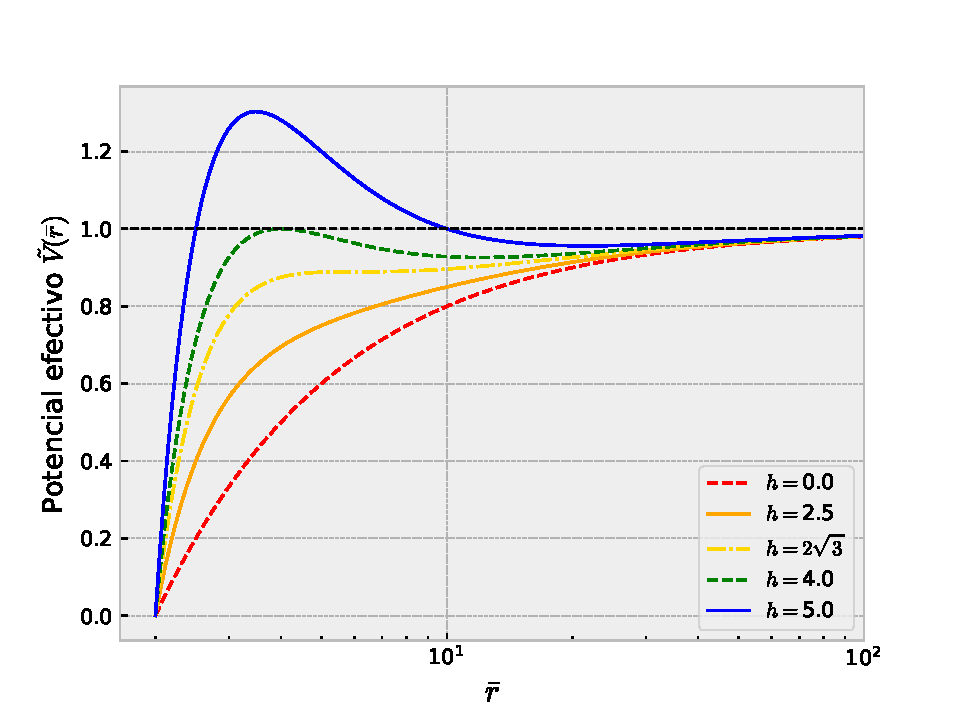
\includegraphics[scale = 0.7]{Potencial_Efectivo.pdf}
    \caption{Potencial efectivo en escala logarítmica en la coordenada radial adimensional $\bar{r} = r/m$.}
    \label{fig:Effective-Potential}
\end{figure}

Notemos que el potencial es cero en $r = 2m$, a diferencia del problema de Kepler.

\section*{Órbitas circulares}

Si $h > 2\sqrt{3}$ y $k^2 = \tilde{V}(r_B)$, tenemos órbitas circulares estables (porque la segunda derivada del potencial es positiva). Determinemos las constantes de movimiento $h = h_c$ y $k = k_c$ apropiadas para tener un movimiento circular con $r = r_c$ conocido. Usando la ecuación \eqref{eq:extremos-locales}, dada para $r_B$, despejemos $h_c$ 
\begin{align}
r_c &= \frac{mh_c^2}{2} \left( 1 + \sqrt{1 - \frac{12}{h_c^2}}\right) \\
r_c&= \frac{mh_c^2}{2} \left( 1 + \frac{1}{h_c} \sqrt{h_c^2 - 12}\right) \\
r_c &= \frac{mh_c}{2} (h_c + \sqrt{h_c^2 - 12})  \\
r_c - \frac{mh_c^2}{2} &= \frac{mh_c}{2} \sqrt{h_c^2-12} \\
r_c^2 - m h_c^2r_c + \CancelTo[\color{red}]{0}{\frac{m^2 h_c^4}{4}} &= \frac{m^2h_c^2}{4} (\CancelTo[\color{red}]{0}{
h_c^2} - 12) \\
r_c^2 - m h_c^2 r_c &= - 3m^2h_c^2 \\
h_c^2 (m r_c - 3m^2) &= r_c^2.  
\end{align}

Por lo tanto,
\colorlet{shadecolor}{green!20}
\begin{shaded}
\begin{equation} \label{eq:circular-orbit-h}
h_c = \frac{r_c}{\sqrt{m(r_c - 3m)}}.
\end{equation}
\end{shaded}

Por otro lado, sabemos que
\begin{equation} \label{eq:circular-orbit-1}
k_c^2 =  \tilde{V}(r_c) = \left(1 - \frac{2m}{r_c} \right) \left(1 + \frac{h_c^2m^2}{r_c^2} \right).
\end{equation}

Entonces, reemplazando \eqref{eq:circular-orbit-h} en \eqref{eq:circular-orbit-1}, obtenemos
\begin{align}
k_c^2 &= \left(1 - \frac{2m}{r_c} \right) \left(1 + \frac{r_c^2m^2}{m(r_c - 3m)r_c^2} \right) \\
&= \left(1 - \frac{2m}{r_c} \right) \left(1 + \frac{m}{r_c - 3m} \right) \\
&= \left(1 - \frac{2m}{r_c} \right) \left(1 + \frac{m}{r_c \left( 1 - \frac{3m}{r_c}\right)} \right) \\
&= \left(1 - \frac{2m}{r_c} \right) \left( \frac{r_c - 3m + m}{r_c \left( 1 - \frac{3m}{r_c}\right)}  \right) \\
&= \frac{\left( 1 - \frac{2m}{r_c}\right)^2}{\left( 1 - \frac{3m}{r_c}\right)}.
\end{align}

Por lo tanto,
\colorlet{shadecolor}{green!20}
\begin{shaded}
\begin{equation} \label{eq:circular-orbit-k}
k_c = \frac{\left( 1 - \frac{2m}{r_c}\right)}{\sqrt{ 1 - \frac{3m}{r_c}}}.
\end{equation}
\end{shaded}

En el documento de la semana 2, encontramos que la constante de movimiento $k$ queda expresada por
\begin{equation}
k = \left( 1 -  \frac{2m}{r}\right) \dot{t}.
\end{equation}

Luego, reemplazando \eqref{eq:circular-orbit-k}, 
\begin{equation}
\frac{\left( 1 - \frac{2m}{r_c}\right)}{\sqrt{ 1 - \frac{3m}{r_c}}} =  \left( 1 -  \frac{2m}{r}\right) \dot{t}_c,
\end{equation}
lo que implica que
\begin{shaded}
\begin{equation} \label{eq:circular-orbit-t}
\dot{t}_c = \frac{1}{\sqrt{1 - \frac{3m}{r_c}}}.
\end{equation}
\end{shaded}

Por otro lado, $hmc = r^2 \sin^2\theta \dot{\varphi} = r^2 \dot{\varphi}$ (recordando que $\theta = \pi/2$). Así, reemplazando \eqref{eq:circular-orbit-h},
\begin{align}
h_c m c &= r_c^2 \dot{\varphi}_c \\
\dot{\varphi}_c &= \frac{mc}{r_c^2} \frac{r_c}{\sqrt{m(r_c - 3m)}} \\
&= \frac{c}{r_c} \sqrt{\frac{m^2}{m(r_c - 3m)}} \\
&= \frac{c}{r_c} \sqrt{\frac{m}{r_c-3m}}.
\end{align}

Esto es,
\begin{shaded}
\begin{equation} \label{eq:circular-orbit-phi}
\dot{\varphi}_c = \frac{c}{r_c} \sqrt{\frac{m}{r_c-3m}}.
\end{equation}
\end{shaded}

Dado que $\dot{t}_c$ y $\dot{\varphi}_c$ son constante, podemos integrar las ecuaciones de movimiento, obteniendo
\begin{equation}
x^{\mu}(\tau) = \left( c\dot{t}_c \tau, r_c, \frac{\pi}{2},\dot{\varphi}_c \tau \right).
\end{equation}

La menor órbita circular estable (innermost stable circular orbit. ISCO), se obtiene, de acuerdo a \eqref{eq:extremos-locales}, en el límite $h\to 2\sqrt{3}$. En este caso, 
\begin{align}
r_c &= \lim_{h\to 2\sqrt{3}} \frac{mh^2}{2} \left(1 + \sqrt{1 - \frac{12}{h^2}} \right) = \frac{m (2\sqrt{3})^2}{2} = 6m, \\
k_{\text{ISCO}} &= \lim_{h\to 2\sqrt{3}} k_c = \frac{\left(1 - \frac{2m}{6m} \right)}{\sqrt{1 - \frac{3m}{6m}}} = \frac{\frac{2}{3}}{\frac{1}{\sqrt{2}}} = \frac{2\sqrt{2}}{3}, \\
\dot{t}_{\text{ISCO}} &= \lim_{h\to 2\sqrt{3}} \dot{t}_c = \frac{1}{\sqrt{1 - \frac{3m}{6m}}} = \sqrt{2}, \\
\dot{\varphi}_{\text{ISCO}} &=  \lim_{h\to 2\sqrt{3}} \dot{\varphi}_c = \frac{c}{6m} \sqrt{\frac{m}{6m-3m}} = \frac{c}{6m \sqrt{3}} = \frac{\sqrt{3}}{18} \frac{c}{m}.
\end{align}

En resumen,
\begin{shaded}
\begin{equation} \label{eq:ISCO}
r_c = 6m, \quad k_{\text{ISCO}} = \frac{2\sqrt{2}}{3}, \quad \dot{t}_{\text{ISCO}} = \sqrt{2}, \quad \dot{\varphi}_{\text{ISCO}} = \frac{\sqrt{3}}{18} \frac{c}{m}.
\end{equation}
\end{shaded}

En el caso newtoniano existen órbitas circulares para cada valor de $r > 0$, en cambio la teoría gravitacional de Einstein predice un límite para la existencia de órbitas circulares estables, para $r_c \geq 6m$.

Notemos que las expresiones calculadas para $h_c$, $k_c$, etc, están bien definidas para $r_c > 3m$, esto se debe a que para $3m < r < 6m$, pueden existir órbitas circulares pero inestables. Por otro lado, para $2m < r < 3m$ no pueden existir órbitas circulares.

En el siguiente \href{https://github.com/AleSaa66/Topicos-RG/blob/main/Semana%203/Semana-3.ipynb}{notebook} encontrará el código del gráfico del potencial y animaciones con de órbitas circulares estables e inestables.
\end{document}
